\lhead[\thepage]{CAPÍTULO \thechapter. PLANIFICACIÓN Y PRESUPUESTO}
\chead[]{}
\rhead[WepSIM: Simulador de un procesador elemental con unidad de control microprogramada\leftmark]{\thepage}
\renewcommand{\headrulewidth}{0.5pt}

\lfoot[]{}
\cfoot[]{}
\rfoot[]{}
\renewcommand{\footrulewidth}{0pt}

%% This is an example first chapter.  You should put chapter/appendix that you
%% write into a separate file, and add a line \include{yourfilename} to
%% main.tex, where `yourfilename.tex' is the name of the chapter/appendix file.
%% You can process specific files by typing their names in at the 
%% \files=
%% prompt when you run the file main.tex through LaTeX.
\chapter{Planificación y presupuesto}
\label{ch:planning_and_budget}
\markboth{}{PLANNING AND BUDGET}

Este capítulo presenta una planificación detallada del proyecto (Sección \ref{sec:planning}, \textit{\nameref{sec:planning}}). Luego, se explican los costes del proyecto (Sección \ref{sec:budget}, \textit{\nameref{sec:budget}}). Al final del capítulo, se explica el entorno socio-económico del proyecto ({Sección \ref{sec:socioeconomic_environment}, \textit{\nameref{sec:socioeconomic_environment}}}).

\section{Planificación}
\label{sec:planning}

Esta sección incluye la planificación completa del proyecto. En primer lugar, se describe la metodología de desarrollo de \gls{software} utilizada. Después, se detalla la duración de cada fase del proyecto, indicando todos los tiempos en un diagrama Gantt.

\subsection{Justificación de la metodología}

Debido a sus características, hemos dividido nuestro proyecto en tres iteraciones:

\begin{itemize}
\item \textbf{Modelo \gls{hardware}:} la primera iteración ha consistido en lograr el modelado del \gls{hardware} que compone el procesador \acrshort{wepsim}. El objetivo de esta fase, ha sido lograr el modelado y funcionamiento básico de cada componente \gls{hardware} por separado.

\item \textbf{Modelo \gls{software}:} esta fase ha consistido en lograr el modelo \gls{software} utilizado en la asignatura Estructura de computadores para la definición del juego de instrucciones y el lenguaje \gls{ensamblador}. El objetivo de esta fase, ha sido lograr interpretar el juego de instrucciones definido y código \gls{ensamblador} definidos por el usuario, generando la memoria de control y memoria principal en el orden correspondiente.

\item \textbf{Kernel del simulador:} esta fase ha consistido en lograr unir el modelo \gls{hardware} y modelo \gls{software}, realizando el kernel del simulador. El objetivo de esta fase, ha sido diseñar e implementar el kernel de simulador encargado de unir el modelo \gls{hardware} y el modelo \gls{software}, generando la simulación y la vista del simulador.
\end{itemize}

Era necesario contar con una metodología iterativa para desarrollar cada una de las fases de manera independiente para unirlas todas en la última etapa y obtener el producto final. Para ello, hemos analizado tres metodologías de desarrollo de \gls{software} diferentes: Prototipado de \gls{software} \cite{grimm1998}, el Modelo en Cascada \cite{hebert1983} y el Modelo en Espiral \cite{boehm1988}. El  Prototipado de \Gls{software} no encaja muy bien en nuestro proyecto, puesto que requiere la construcción de un prototipo de sofware en poco tiempo. El Modelo en Cascada es un proceso de diseño secuencial, utilizado en procesos de desarrollo de \gls{software} en el cual el progreso es visto como un flujo constante hacia abajo (como una cascada) a través de diferentes fases. El problema con esta metodología es que no permite iteraciones dentro del desarrollo del \gls{software}. Finalmente, el Modelo en Espiral permitió dividir el proyecto en diferentes iteraciones. Este modelo, combina las fortalezas de los otros dos modelos (simplicidad y flexibilidad), utilizando además un proceso iterativo. Aunque este modelo es más lento que los dos anteriores, nos permitió aplicar diferentes iteraciones por lo que decidimos aplicarlo a todo el proceso.

\subsection{Ciclo de vida}

El proceso de desarrollo del ciclo de vida del proyecto ha seguido el Modelo de ciclo de vida en Espiral \cite{boehm1988}. La Figura \ref{fig:spiral_model} muestra el Modelo en Espiral usando un esquema.

\begin{figure}[htbp]
 	\centering
 	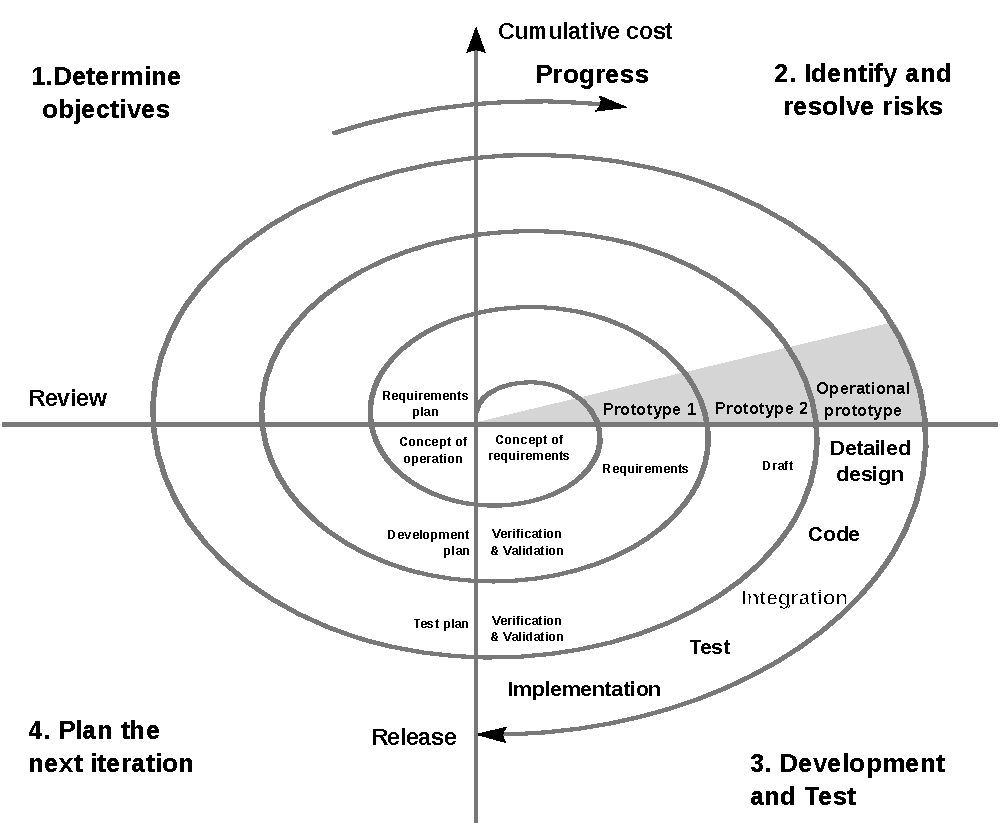
\includegraphics[width=12cm]{figures/spiral_model}
 	\caption{Modelo en Espiral (Boehm, 2000).}
	\label{fig:spiral_model}
\end{figure}

El modelo en Espiral tiene cuatro fases, que se repiten durante las diferentes iteraciones del modelo. Estas fases son:

\begin{itemize}
\item \textbf{Planificación} (\emph{``Determine objectives''} en Figura \ref{fig:spiral_model}): Se reúnen los requisitos de los usuarios, se realiza un estudio de factibilidad del sistema y se determinan los objetivos de iteración.

\item \textbf{Análisis} (\emph{``Identify and resolve risks''} en Figura \ref{fig:spiral_model}): Se realiza un análisis completo de los requisitos y se identifican los posibles riesgos. Esta fase termina con un diseño básico.

\item \textbf{Desarrollo y Pruebas} (\emph{``Development and Test''} en Figura \ref{fig:spiral_model}): Se lleva a cabo la implementación del código. Se realizan los casos de prueba y los resultados de la prueba.

\item \textbf{Evaluación} (\emph{``Plan the next iteration''} en Figura \ref{fig:spiral_model}): 
Los clientes evalúan el \gls{software} y proporcionan sus comentarios. En este caso, el estudiante intenta obtener la aprobación del supervisor. Esta es la \textit{tarea crítica} del ciclo de vida, ya que solo podemos pasar a la siguiente iteración del Modelo de ciclo de vida Espiral si esta tarea es aprobada.

\end{itemize}

Cada fase comienza con un objetivo de diseño y termina con el cliente (el supervisor) revisando el progreso hasta ahora. Como se explicó anteriormente, hemos dividido el desarrollo de \gls{software} en tres iteraciones: modelo \gls{hardware}, modelo \gls{software}, y kernel del simulador. En la última iteración, el \gls{software} completo debe someterse a pruebas exhaustivas para validar el simulador.

\subsection{Tiempo estimado}

El diagrama de Gantt (Figura \ref{fig:gantt}) muestra todas las tareas realizadas durante el desarrollo del proyecto. El proyecto comenzó el 2 de noviembre de 2015 y finalizó el 30 de diciembre de 2016, lo que supone un total de casi 13 meses de trabajo (305 días laborables). Durante este tiempo, he trabajado de lunes a viernes, durante cuatro horas al día, haciendo un total de 1.220 horas trabajadas.

El diagrama de Gantt muestra todas las tareas realizadas en cada iteración del modelo de ciclo de vida espiral. Recuerde que las tres iteraciones fueron: Modelo \gls{hardware}, Modelo \gls{software} y kernel del simulador. Además de las tareas (fases) mencionadas anteriormente (Planificación, Análisis, Desarrollo y Prueba, y Evaluación), hemos incluido la tarea de Documentación al final de cada iteración. La tarea de documentación ha consistido principalmente en la redacción de este trabajo fin de grado.

\begin{figure}[htbp]
 	\centering
 	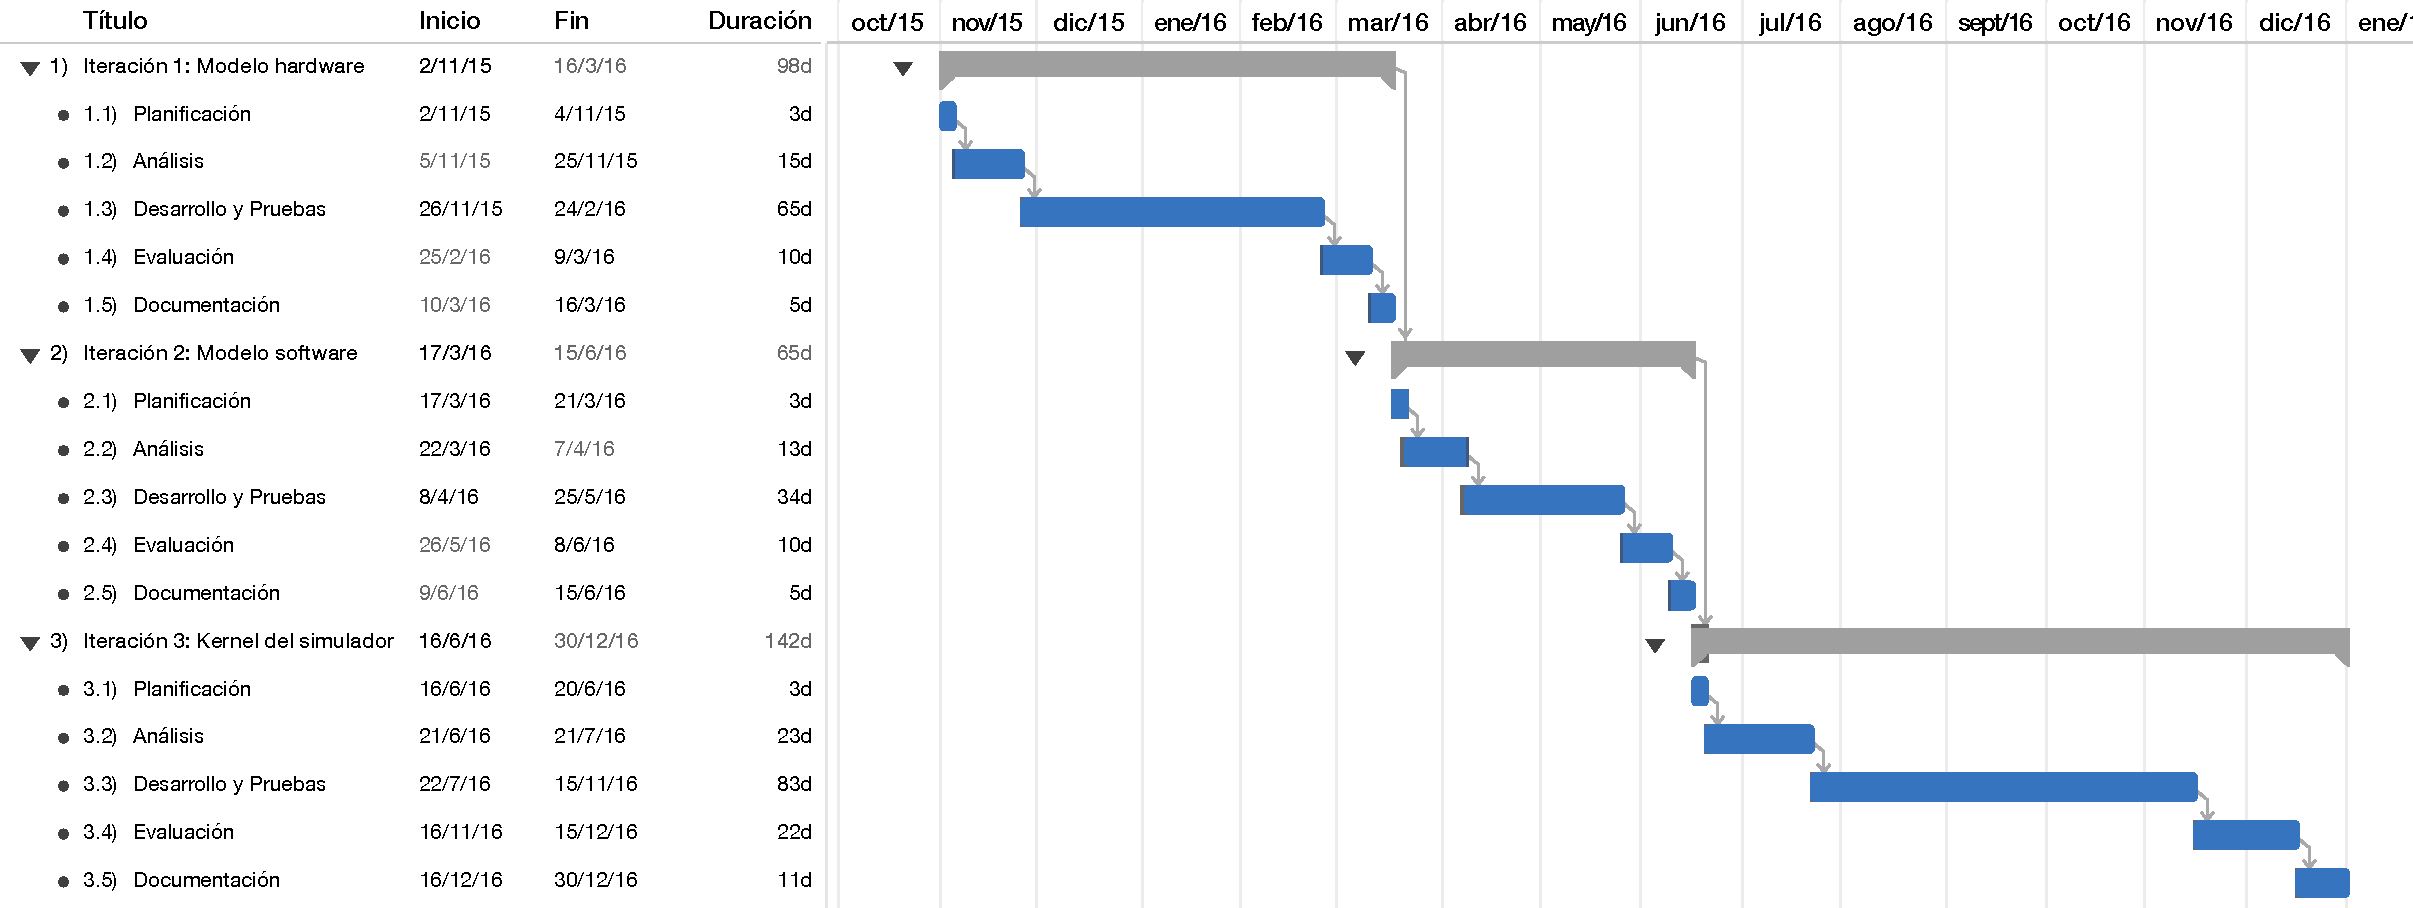
\includegraphics[width=16.5cm]{figures/ganttFuente}
 	\caption{Diagrama Gantt.}
	\label{fig:gantt}
\end{figure}

\section{Presupuesto}
\label{sec:budget}

Esta sección detalla el presupuesto general del proyecto. Por un lado, presentamos los costes del proyecto y, por otro lado, damos a conocer la oferta presentada al cliente.

\subsection{Coste del proyecto}

La Tabla \ref{tab:project_information} resume las principales características del proyecto, incluido el presupuesto total.

\begin{center}
\ra{1.2}
\begin{table*}[htbp]
\centering
\caption{Información del Proyecto.}
\begin{tabular}{@{}p{3.5cm} p{9cm}@{}} 
\toprule
\multicolumn{2}{c}{\textbf{\textit{Información del Proyecto}}}\\
\midrule
\textbf{Título} 					& \acrshort{wepsim}: Simulador de un procesador elemental con unidad de control microprogramada \\
\midrule
\textbf{Autor} 					& Javier Prieto Cepeda \\
\midrule
\textbf{Departamento} 				& Departamento de Informática \\
\midrule
\textbf{Fecha de inicio}				&2 de noviembre de 2015 \\
\midrule
\textbf{Fecha de finalización}				& 30 de diciembre de 2016 \\
\midrule
\textbf{Duración} 				& 13 meses \\
\midrule
\textbf{Ratio de costes indirectos} 	& 20 \% \\
\midrule
\textbf{Presupuesto total} 			& 51.860,96 \euro \\
\bottomrule
\end{tabular}
\label{tab:project_information}
\end{table*}
\end{center}

\vspace{5cm}

A continuación se desglosa el presupuesto total del proyecto.

\subsubsection{Costes Directos}

En esta parte se presentan los costes directos del proyecto. La Tabla \ref{tab:dhrc} muestra los costes directos causados por los costes de personal, sobre la base de la planificación presentada en la sección anterior. El tutor y el estudiante han desempeñado los siguientes roles:

\begin{itemize}

\item \textbf{Tutor:} Jefe de Proyecto.

\item \textbf{Estudiante:} Analista, Desarrollador, Tester.

\end{itemize} 

\begin{center}
\ra{1.2}
\begin{table*}[htbp]
\centering
\caption{Costes de recursos humanos.}
\begin{tabular}{@{}p{3cm} R{3.5cm} R{2.2cm} R{2.4cm}@{}} 
\toprule
\textbf{Categoría} & \textbf{Coste por hora (\euro)} & \textbf{Horas} & \textbf{Total (\euro)} \\
\midrule
Jefe de Proyecto					& 60 						& 65			& 3.900 \\
Analista			 				& 35							& 269		& 9.415 \\
Desarrollador		 				& 35							& 523		& 18.305 \\
Tester		 					& 25							& 428		& 10.700 \\
\midrule
\textbf{\textit{Total}}			&							&			& \textbf{42.320,00}\\
\bottomrule
\end{tabular}
\label{tab:dhrc}
\end{table*}
\end{center}

La Tabla \ref{tab:dec} muestra los costes directos causados por la adquisición y uso del equipo. El coste amortizado, C, es calculado utilizando la siguiente fórmula:

\begin{equation}
  C = \frac{d \cdot c \cdot u}{D}
\label{eq:costs}
\end{equation}

Donde:

\begin{itemize}

\item \textbf{C:} Coste amortizado. Es equivalente al valor amortizado.

\item \textbf{d:} Tiempo que el equipamiento ha sido utilizado.

\item \textbf{c:} Coste del equipamiento. 

\item \textbf{u:} Dedicación al proyecto. Porcentaje del tiempo que el equipamiento ha sido utilizado.

\item \textbf{D:} Periodo de amortización del equipamiento.

\end{itemize}

\begin{center}
\ra{1.2}
\begin{table*}[htbp]
\centering
\caption{Costes de equipamiento.}
\begin{tabular}{@{}p{2.5cm} C{1.6cm} C{2.1cm} C{2.1cm} C{2.7cm} C{2.3cm}@{}} 
\toprule
\textbf{Concepto} & \textbf{Coste, c (\euro)} & \textbf{Dedicación, u (\%)} & \textbf{Dedicación, d (meses)} & \textbf{Amortización, D (meses)} & \textbf{Coste amortizado, C (\euro)}\\
\midrule
\acrshort{pc} sobremesa		 			& \multicolumn{1}{r}{799,99}		& \multicolumn{1}{r}{100}		& \multicolumn{1}{r}{13} 		& 	\multicolumn{1}{r}{36}	& 	\multicolumn{1}{r}{288,89} \\
Portátil 						& \multicolumn{1}{r}{529,99} 	& \multicolumn{1}{r}{25}			& \multicolumn{1}{r}{13} 		& 	\multicolumn{1}{r}{36}	& 	\multicolumn{1}{r}{47,85} \\
\acrshort{arcos} Mirlo					& \multicolumn{1}{r}{1.979,99}	& \multicolumn{1}{r}{50}			& \multicolumn{1}{r}{7} 		& 	\multicolumn{1}{r}{60}	& 	\multicolumn{1}{r}{115,50} \\
Impresora						& \multicolumn{1}{r}{79,99}		& \multicolumn{1}{r}{5}			& \multicolumn{1}{r}{4}		& 	\multicolumn{1}{r}{60}	& 	\multicolumn{1}{r}{0,27} \\
\midrule
\textbf{\textit{Total}}		&			&			& 			& &  \multicolumn{1}{r}{\textbf{452,51}}\\
\bottomrule
\end{tabular}
\label{tab:dec}
\end{table*}
\end{center}

Además, el equipo presentado en la Tabla \ref{tab:dec} es detallado a continuación:

\begin{itemize}

\item \textbf{\acrshort{pc} sobremesa:} All in One - Asus Z220ICUK, 21.5'', i5-6400T, 8GB, 1TB)		

\item \textbf{Portátil:} Toshiba L50D-C-19D, A10-8700P, 8GB \gls{ram} and 1TB.

\item \textbf{\acrshort{arcos} Mirlo:} Servidor utilizado por el grupo de investigación \acrshort{arcos}. 32GB \gls{ram} y 8 procesadores  i7 a 2.67GHz cada uno.

\item \textbf{Impresora:} Brother DCP-1510.

\end{itemize}

Otros costes directos se muestran en la Tabla \ref{tab:odc}. Estos costes consisten en material de oficina, un tóner para la impresora y el abono transporte mensual. El material de oficina incluye: lápices, bolígrafos, cuadernos, papel y marcadores.



\begin{center}
\ra{1.2}
\begin{table*}[htbp]
\centering
\caption{Otros costes directos.}
\begin{tabular}{@{}p{5cm} R{3.5cm}@{}} 
\toprule
\textbf{Concepto} & \textbf{Coste (\euro)} \\
\midrule
Material de oficina				& 112,98				\\
Toner (x1) 			 			& 71,99				\\
Abono transporte (x13) 		& 260				\\
\midrule
\textbf{\textit{Total}}		&	\textbf{444,97}  	\\
\bottomrule
\end{tabular}
\label{tab:odc}
\end{table*}
\end{center}

\subsubsection{Resumen de costes}

La Tabla \ref{tab:cs} muestra el resumen completo de los costes del proyecto. Los costes indirectos (20\% de los costes directos) consisten en las facturas de electricidad y agua, teléfono, acceso a internet, etc.

\begin{center}
\ra{1.2}
\begin{table*}[htbp]
\centering
\caption{Resumen de costes.}
\begin{tabular}{@{}p{5cm} R{5cm}@{}} 
\toprule
\multicolumn{2}{c}{\textbf{\textit{Resumen de costes}}}\\
\midrule
\textbf{Recursos humanos} 				& 42.320,00 \euro \\
\textbf{Equipamiento} 						& 452,51 \euro \\
\textbf{Otros costes directos} 				& 444,97 \euro \\
\textbf{Costes indirectos}					& 8.643,50 \euro \\
\midrule
\textbf{\textit{Presupuesto total}}			& \textbf{51.860,98} \euro \\
\bottomrule
\end{tabular}
\label{tab:cs}
\end{table*}
\end{center}

El presupuesto total de este proyecto asciende a \textbf{51.860,98 \euro \ (cincuenta y uno mil ochocientos sesenta euros y noventa y ocho céntimos)}.

\subsection{Oferta de Proyecto Propuesta}

La Tabla \ref{tab:offer} muestra la propuesta de oferta detallada. Esta oferta incluye los riesgos estimados (20\%), los beneficios esperados (15\%), y el Impuesto de Valor Agregado (\gls{iva}), que corresponde al 21\% \cite{iva2012}. Después de aplicar todos estos conceptos, la cantidad final para este proyecto en caso de venta a un cliente de terceros es \textbf{86.597,46 \euro \ 
(Ochenta y seis mil quinientos noventa y siete euros y cuarenta y seis céntimos)}.

\begin{center}
\ra{1.2}
\begin{table*}[htbp]
\centering
\caption{Oferta propuesta.}
\begin{tabular}{@{}p{2.5cm} R{2.8cm} R{3.1cm} R{3.5cm}@{}} 
\toprule
\multicolumn{4}{c}{\textbf{\textit{Oferta propuesta}}}\\
\midrule
\textbf{Concepto} & \textbf{Incremento (\%)} & \textbf{Valor Parcial (\euro)} & \textbf{Coste agregado (\euro)} \\
\midrule
Costes del proyecto				& - 			& 51.860,98		& 51.860,98 \\
Riesgos			 				& 20			& 10.372,20		& 62.233,17 \\
Beneficios		 				& 15			& 9.334,98		& 71.568,15 \\
IVA		 					& 21			& 15.029,31		& 86.597,46 \\
\midrule
\textbf{\textit{Total}}		&			&			& \textbf{86.597,46}\\
\bottomrule
\end{tabular}
\label{tab:offer}
\end{table*}
\end{center}

\section{Entorno socio-económico}
\label{sec:socioeconomic_environment}



Gracias al trabajo realizado en este proyecto, se consiguen las siguientes mejoras que ahorran costes en la enseñanza de ``Estructura de Computadores'' y mejoran la calidad de la misma:

\begin{itemize}

\item \textbf{\textit{Mejor aprovechamiento del tiempo dedicado al laboratorio de prácticas}}, debido al uso de una herramienta que integra todos los conceptos necesarios para las prácticas, evitando aprender diferentes entornos.

\item \textbf{\textit{Ampliar el tiempo de realización de las prácticas}}, ya que al permitir el uso en diferentes dispositivos (\emph{smartphones, tablets, etc.}) se aumentan los momentos aptos para realizar las prácticas.

\item \textbf{\textit{Aumento de los casos prácticos}}, dado que es posible trabajar con diferentes juegos de instrucciones, diferentes tipos de procesadores, diferentes elementos \gls{hardware}, etc.

\item \textbf{\textit{Colaboraciones con instituciones docentes}}, ya que al ser una herramienta con licencia de código abierto favorece las colaboraciones entre diferentes instituciones promocionando a la universidad mediante las herramientas que desarrolla. Además, esta herramienta puede ser integrada con facilidad en \emph{SPOCs} y \emph{MOOCs}.

\item \textbf{\textit{Disponer de la solución de forma gratuita}}, ayuda tanto a otras universidades que deseen hacer uso de la herramienta como a los estudiantes a ahorrar dinero puesto que no tienen que adquirir material adicional para la realización de las prácticas de laboratorio.

\end{itemize}

Por tanto, \acrshort{wepsim} ayuda a optimizar el tiempo dedicado por los estudiantes al estudio de la asignatura puesto que aumenta la posibilidad de disponer de tiempo para la realización de la práctica aumenta y el tiempo invertido en el aprendizaje de entornos de desarrollo disminuye, al disponer únicamente de un único entorno de desarrollo. De esta forma:

\begin{equation}
 Tent + \sum_{i=1}^{n}((Tefec_{i} + Tperd_{i}) + Tteor_{i}) < \sum_{j=1}^{n}((Tefec_{j} + Tperd_{j}) + Tteor_{j}+ Tent_{j})
\label{eq:tiempo_invertido}
\end{equation}

Donde:

\begin{itemize}

\item \textbf{\textit{$Tent_{x}$:}} Tiempo invertido en el aprendizaje del entorno de desarrollo, siendo x cada una de las prácticas de laboratorio.

\item \textbf{\textit{$Tefec_{x}$:}} Tiempo efectivo en el desarrollo de la práctica, siendo x cada una de las prácticas de laboratorio.

\item \textbf{\textit{$Tperd_{x}$:}} Tiempo perdido por dependencias del entorno de desarrollo, siendo x cada una de las prácticas de laboratorio.

\item \textbf{\textit{$Tteor_{x}$:}} Tiempo invertido al estudio de la teoría necesaria para el desarrollo de la práctica, siendo x cada una de las prácticas de laboratorio.

\item \textbf{\textit{n:}} Número de prácticas de laboratorio en la asignatura.

\end{itemize}

De este modo en la ecuación \ref{eq:tiempo_invertido} podemos observar como el tiempo total invertido en la realización de las prácticas por los estudiantes es menor haciendo uso de esta herramienta (\emph{término a la izquierda de la desigualdad}) que con el sistema anterior (\emph{término a la derecha de la desigualdad}), que hacía uso de diferentes herramientas. En el nuevo sistema, se aprende un único entorno de desarrollo (\emph{Tent}) y además, el tiempo pérdido por dependencias del entorno (\emph{Tperd}) se ve reducido debido a la portabilidad que ofrece la nueva herramienta.

Con respecto al aumento de los casos prácticos, un ejemplo sería mostrar al estudiante el impacto energético que supone una programación eficiente, pudiendo ser comparado entre diferentes computadores. Esto es debido a que \acrshort{wepsim} simula la microprogramación de un computador y la programación en lenguaje \gls{ensamblador}, pudiendo hacer visible el coste a bajo nivel de unas malas prácticas de programación. El objetivo, es concienciar a los estudiantes de la importancia que tiene la optimización y eficiencia en el uso de los recursos de un computador, puesto que uno de los retos de la comunidad científica es diseñar sistemas cada vez más eficientes energéticamente, de forma que en un futuro estas técnicas sean llevadas a cabo realizando sistemas más eficientes.

Con todo ello, los estudiantes están más capacitados con los mismos recursos tanto materiales como de tiempo, sin la necesidad de adquirir material adicional para la realización de los casos prácticos.


\iffalse
% resumen
Gracias al trabajo realizado en este proyecto, se consiguen diferentes mejoras, que ahorran costes en la enseñanza y mejoran la calidad de la misma:

\begin{itemize}
\item Mejor aprovechamiento del tiempo dedicado al laboratorio de practicas, debido a que en vez de aprender diferentes entornos para prácticas, únicamente se aprende uno que integra todo.

\item Ampliar el tiempo en el que se pueden realizar las prácticas, ya que al permitir el uso de diferentes dispositivos (smartphones, tablets) los momentos para realizar las prácticas se aumentan.

\item Ampliación de los casos prácticos, dado que es posible trabajar con distintos juegos de instrucciones, diferentes tipos de procesadores, diferentes elementos \gls{hardware}, etc. (Como ejemplo del punto 3, metemos energía y optimización).

\item Colaboraciones con instituciones docentes, ya que al ser una herramienta con licencia de código abierto, favorece esa colaboración promocionando la universidad mediante las herramientas que desarrolla.
Esta herramienta puede ser integrada con facilidad en spoc's (versión del moc en la universidad, privados) y mooc's (masivos) para la realización de los casos prácticos.

\item Disponer de la solución gratis, ayuda tanto a otras universidades que quieran hacer uso de ella, como a los estudiantes ahorrar dinero al no tener que adquirir diferentes componentes para la realización de las prácticas de laboratorio.

\end{itemize}

Resumen primeros puntos.

Con todo ello, los estudiantes están más capacitados con los mismos recursos tanto materiales como de tiempo, sin la necesidad de adquirir herramientas para la realización de los casos prácticos.

costes socioeconomicos de la situación actual de la asignatura

En la enseñanza de estructura de computadores son importantes las practicas. Habitualmente el tiempo total dedicado a la asiguntura es:teoria del entorno + aprendizaje de entorno + realización de practica + tiempo teoría. Para realizar las practicas se necesitan unos medios especificos, ya sea mediante el uso de recursos compartidos en la universidad en los laboratorios o mediante la adquisición de los componentes necesarios, cosa que para estudiantes con recursos limitados es malo, y para aquellos que no pueden tener asistir por diferentes motivos (trabajo, aprendizaje a distancia).

Cada una de estas caracteristicas tienen un impacto. Para mejorar el impacto anterior, \acrshort{wepsim} ha trabajo en mejorar estas caracteristicas. Integración de microprogramación y programacion en \gls{ensamblador} en una misma herramienta, reduciendo el tiempo de aprendizaje de entornos de trabajo. 

El diseño modular da mayor flexibilidad para poner al estudiante en diferentes situaciones que antes no tenia. La alternativa sería comprar distintos tipos de procesadores y distintos tipos de componentes, con un coste elevado tanto de adquisición como de mantenimiento.

Gracias a ser portable y no requerir instalación, el estudiante no precisa de una plataforma concreta para la realización de  las prácticas, pudiendo utilizar un smartphone o tablet, con la movilidad que proporciona, permitiendo su uso fuera de los laboratorios de prácticas. Además, se incluye la ventaja de facilitar su uso a quienes por diferentes motivos, no pueden asistir a clase (por enfermedad, ...), de forma que pueden hacer uso de la herramienta sin limitarse al tiempo disponible para asisitir a la universidad.

Otro aspecto positivo del diseño multiplataforma de esta herramienta, es el aprovechamiento del tiempo libre que en ocasiones los estudiantes tienen en los trayectos al centro de estudios. Anteriormente, al utilizar herramientas específicas para \acrshort{pc}, suponían que si no se disponía de un computador, no se podía utilizar la plataforma. De esta manera, el estudiante puede aprovechar cualquier instante de tiempo disponible para hacer uso de la herramienta, puesto que tan solo necesita de un dispositivo con navegador web.



Como se ha comentado en capítulos anteriores, \acrshort{wepsim} puede apoyar la enseñanza en Estructura y Arquitectura de Computadores. Esto significa que los profesores de estas asignaturas pueden utilizar esta herramienta como refuerzo en las explicaciones del temario para mostrar de forma visual y práctica a los estudiantes el comportamiento de un procesador elemental. Además, sirve para que los estudiantes puedan desarrollar las prácticas de estas asignaturas sin la necesidad de utilizar diferentes herramientas, evitando la pérdida de tiempo que esto supone y permitiendo a los estudiantes dedicar el mayor tiempo posible a la realización de los ejercicios. Este ahorro de tiempo, tiene un impacto en los estudiantes a la hora de minimizar el tiempo invertido en la realización de prácticas, de forma que la mayor parte del tiempo dedicado a la asignatura sea útil y sirva para comprender mejor el funcionamiento de un computador, sirviendo de base en el resto de la trayectoria académica de los estudiantes y mejorando su rendimiento.

Debido al diseño modular realizado de este simulador, \acrshort{wepsim} permite la especificación tanto de diferentes juegos de instrucciones como de diferentes modelos \gls{hardware}. Esto supone un gran avance  en el área docente, puesto que permite el uso de una misma herramienta para la enseñanza y simulación de diferentes dispositivos. Anteriormente se invertía mucho dinero para que los estudiantes pudieran realizar prácticas con diferentes tipos de procesadores, ya que se debían de adquirir los diferentes componentes \gls{hardware} necesarios para la realización de las prácticas. Con \acrshort{wepsim} este concepto cambia, puesto que modelando el comportamiento del computador deseado, puede ser utilizado para diferentes tipos de prácticas, evitando costes de adquisición y mantenimiento y permitiendo una mayor variedad de opciones a la hora de diseñar las prácticas.

Gracias al uso de este simulador en el ámbito docente, se puede mostrar el impacto energético que supone una programación eficiente. Esto es debido a que \acrshort{wepsim} es un simulador de microprogramación y programación en \gls{ensamblador}, pudiendo hacer visible el coste a bajo nivel de unas malas prácticas de programación. El objetivo, es concienciar a los estudiantes de la importancia que tiene la optimización y eficiencia en el uso de los recursos de un computador, puesto que uno de los retos de la comunidad científica es diseñar sistemas cada vez más eficientes energéticamente, de forma que en un futuro estas técnicas sean llevadas a cabo realizando sistemas más eficientes.

Por último, es necesario destacar el impacto que supone que \acrshort{wepsim} tenga licencia de código abierto. Esto supone que las universidades y centros docentes que quieran utilizar la herramienta, puedan hacerlo sin ningún tipo de coste, con el ahorro económico que supone la utilización de una herramienta de estas características. Además, gracias a este tipo de licencia, se favorece un entorno de colaboración entre diferentes universidades, de forma que se puedan añadir nuevos módulos a la herramienta sin coste económico para la comunidad docente.

\fi